\documentclass{article} % For LaTeX2e
\usepackage{nips12submit_e,times}
\usepackage{amsfonts}
\usepackage{amssymb}
\usepackage{amsmath}
\usepackage{amsopn}
\usepackage{amsthm}
\usepackage[pdftex]{graphicx}
\usepackage{mathrsfs}

\title{An Alternative Kernel Method for the Two-Sample Problem}

\author{
Nelson C.~Ray%\thanks{ Use footnote for providing further information
%about author (webpage, alternative address)---\emph{not} for acknowledging
%funding agencies.} \\
Department of Statistics\\
Stanford University\\
Stanford, CA 94305 \\
\texttt{ncray@stanford.edu} \\
\And
Susan P.~Holmes \\
Department of Statistics\\
Stanford University\\
Stanford, CA 94305 \\
\texttt{susan@stat.stanford.edu} \\
}

% The \author macro works with any number of authors. There are two commands
% used to separate the names and addresses of multiple authors: \And and \AND.
%
% Using \And between authors leaves it to \LaTeX{} to determine where to break
% the lines. Using \AND forces a linebreak at that point. So, if \LaTeX{}
% puts 3 of 4 authors names on the first line, and the last on the second
% line, try using \AND instead of \And before the third author name.

\newcommand{\fix}{\marginpar{FIX}}
\newcommand{\new}{\marginpar{NEW}}
\providecommand{\norm}[1]{\lVert#1\rVert}
\newtheorem{thm}{Theorem}[section]
\newtheorem{cor}[thm]{Corollary}
\newtheorem{lem}[thm]{Lemma}

\theoremstyle{remark}
\newtheorem{rem}[thm]{Remark}
\newtheorem{mydef}{Definition}

%\nipsfinalcopy % Uncomment for camera-ready version

\begin{document}


\maketitle

\begin{abstract}
We present an alternative kernel method for the two-sample problem
that is based on Friedman's approach of using any binary
classification learning machine to score the data.  When the learning
machine is chosen to be a support vector machine, we show that this
approach is a generalization of the permutation $t$-test.  Moreover, due
to the permutation procedure, the significance level of the test is
exactly $\alpha$ by construction.  This advantage is apparent with small
samples when compared with earlier tests based on the Maximum Mean
Discrepancy.  We show how to extend our test to situations with
heterogeneous data and the problem of data integration.
\end{abstract}

\section{Introduction}
The two-sample problem addresses the issue of comparing samples from
two possibly different probability distributions.  They range from
simple parametric, location alternative tests on univariate data such as the
$t$-test to more general non-parametric, ``consistent'' tests, which
have power against all alternatives.  Many options exist for vectorial
data, and kernels provide an enticing avenue for extensions to more
general data types.  

The two-sample problem is also widely prevalent: diet creators may
wish to determine whether their regimens are efficacious.  Biologists
would like to know whether gene expression levels on a set of genes
differ between cancer and control groups.  Further uses for two-sample
testing include authorship validation.  Given two sets of documents,
is the hypothesis of a single author consistent with the data?  

The two-sample problem is generally posed in the following fashion: $\{
\mathbf{x}_i\}_1^n$ are drawn from $p(\mathbf{x})$ and
$\{\mathbf{y}_i\}_1^m$ are drawn from $q(\mathbf{y})$, where $\mathbf{x}_i,
\mathbf{y}_i \in \mathbb{R}^p$. The goal is to test $H_0:
p(\mathbf{x}) = q(\mathbf{y})$ against $H_A: p(\mathbf{x}) \neq
q(\mathbf{y})$. An ideal test should have power against all
alternatives. That is, as $n,m \to \infty$, the test
will always reject when $p \neq q$ for any non-zero significance level
$\alpha$. 

\section{The Friedman Two-Sample Test}
Friedman proposed the following approach to the two-sample problem
\cite{friedman30908multivariate}:

For $\{\mathbf{x}_i\}_1^N$ drawn from $p(\mathbf{x})$ and
$\{\mathbf{z}_i\}_1^M$ drawn from $q(\mathbf{x})$, we would like to
test $\mathcal{H}_A$: $p \neq q$ against $\mathcal{H}_0$: $p = q$.
\begin{enumerate}
\item Pool the two samples $\{\mathbf{u}_i\}_1^{N+M} =
  \{\mathbf{x}_i\}_1^{N} \cup \{\mathbf{z}_i\}_1^{M}$ to create a
  predictor variable training set. 
\item Assign a response value $y_i = 1$ to the observations from the
  first sample ($1 \leq i \leq N$) and $y_i = -1$ to the observations
  from the second sample ($N + 1 \leq i \leq N+M)$. 
\item Apply a binary classification learning machine to the training
  data to produce a scoring function $f(\mathbf{u})$ to score each of
  the observations $\{s_i = f(\mathbf{u}_i)\}_1^{N+M}$. 
\item Calculate a univariate two-sample test statistic $\hat{t} =
  T(\{s_i\}_1^N,\{s_i\}_{N+1}^{N+M})$. 
\item Determine the permutation null distribution of the above
  statistic to yield a p-value. 
\item The test rejects $\mathcal{H}_0$ at significance level $\alpha$
  if $p < \alpha$.
\end{enumerate}

The Friedman Test is a simple, elegant idea that leverages the
many advancements made over the past several decades in the fields of
prediction and classification and applies them to the problem of
two-sample testing.  In short, as long as there exists a learning
machine for the problem at hand, the Friedman Test provides a recipe
for turning that learning machine into a two-sample test.  This
immediately yields two-sample tests for many kinds of data, including
all types for which kernels have been defined.
But there still remains some choice in the scoring
function $F(\mathbf{u})$.  It must be flexible enough to discriminate
between the potential distributional differences of the problem at
hand.   

Because of the permutation design, the test has level $\alpha$ by
construction.  Recall that the level of significance of a test,
$\alpha$, is the probability that we reject the null hypothesis given
that the null hypothesis is true, also known as type I error.  Given
a threshold $\alpha$, we wish to minimize the type II error, accepting
the null hypothesis given that the alternative hypothesis is true.
Equivalently, we wish to maximize the power, one minus the type II
error \cite{lehmann2005testing}.
The downside of the permutation design, of course, is that any computational cost
is na\"\i vely multiplied by the number of permutations.  However,
there are many situations for which the cost is sublinear in the
number of permutations.  For instance, pre-computing the kernel matrix
yields substantial savings.

\section{SVM}
We experienced better computational results with Support Vector
Machine (SVM) regression rather
than classification in the {\bf R} \cite{cran} package {\bf kernlab} \cite{kernlab}.

Recall that SVM regression solves the following problem \cite{scholkopf2002learning}:
\begin{equation*}
\begin{aligned}
& \underset{\mathbf{w}\in\mathcal{H},\mathbf{\xi}^{(*)}\in\mathbb{R}^m,b\in\mathbb{R}}{\text{minimize}}
& &\tau(\mathbf{w},\mathbf{\xi}^{(*)}=\frac{1}{2}\norm{\mathbf{w}}^2+C\sum_{i=1}^M(\xi_i+\xi_i^*) \\
& \text{subject to}
& & f(\mathbf{x}_i)-y_i \leq \epsilon +\xi_i\\
&&& y_i-f(\mathbf{x}_i) \leq \epsilon+\xi_i^* \\
&&& \xi_i,\xi_i^*\geq0 \qquad \qquad \quad \text{for all } i=1,\ldots,m.
\end{aligned}
\end{equation*}

The dual problem is
\begin{equation*}
\begin{aligned}
& \underset{\mathbf{\alpha},\mathbf{\alpha}^*\in\mathbb{R}^m}{\text{maximize}}
& & -\epsilon
\sum_{i=1}^m(\alpha_i^*+\alpha_i)+\sum_{i=1}^m(\alpha_i^*-\alpha_i)y_i
-\frac{1}{2}\sum_{i,j=1}^m(\alpha_i^*-\alpha_i)(\alpha_j^*-\alpha_j)k(x_i,x_j) \\
& \text{subject to}
& & 0\leq\alpha_i,\alpha_i^*\leq C \text{ for all } i=1,\ldots,m,
\text{ and } \sum_{i=1}^m(\alpha_i-\alpha_i^*)=0.
\end{aligned}
\end{equation*}

Finally, the solution is given by
\begin{equation*}
  f(x)=\sum_{i=1}^m(\alpha_i^*-\alpha_i)k(x_i,x)+b.
\end{equation*}

\begin{thm}
  The Friedman Support Vector Machine Procedure (FSVMP) generalizes the two-sample permutation $t$-test. Namely, the two procedures are equivalent with univariate data and a linear kernel.
\end{thm}

\begin{proof}
  \begin{equation*}
    f(x)=\sum_{i=1}^m(\alpha_i^*-\alpha_i)k(x_i,x)+b =
    \sum_{i=1}^m(\alpha_i^*-\alpha_i)x_ix+b = wx+b
  \end{equation*}
  since we have univariate data and a linear kernel.
  Therefore, the SVM score is simply a linear transformation of the
  data.  Welch's $t$-statistic is given by
  \begin{equation*}
    T(\{x_i\}_1^N,\{z_i\}_1^M) = \frac{\bar{x}-\bar{z}}{\sqrt{\frac{s_X^2}{N}+\frac{s_z^2}{M}}}
  \end{equation*}
  where 
  \begin{equation*}
    \bar{x}=\frac{1}{N}\sum_{i=1}^N x_i \text{ and }
    s_X^2= \frac{1}{N-1}\sum_{i=1}^N(x_i-\bar{x})^2.
  \end{equation*}
  Let $z=f(x)=wx+b$ and note that 
  \begin{equation*}
    \bar{z}=\frac{1}{N}\sum_{i=1}^N z_i = \frac{w}{N}\sum_{i=1}^N x_i
    + b = w\bar{x}+b
  \end{equation*}
  and 
  \begin{equation*}
    s_Z^2= \frac{1}{N-1}\sum_{i=1}^N(z_i-\bar{z})^2= \frac{1}{N-1}\sum_{i=1}^N(wx_i+b-w\bar{x}+b)^2=w^2s_X^2.
  \end{equation*}
  Therefore, 
  \begin{equation*}
    T(\{f(x_i)\}_1^N,\{f(z_i)\}_1^M) =
    \frac{w\bar{x}+b-w\bar{z}+b}{|w|\sqrt{\frac{s_X^2}{N}+\frac{s_z^2}{M}}}
    = \text{sign}(w) T(\{x_i\}_1^N,\{z_i\}_1^M).
  \end{equation*}
  Since we are interested in two-sided testing, we consider
  \begin{equation*}
    |T(\{f(x_i)\}_1^N,\{f(z_i)\}_1^M)| = |T(\{x_i\}_1^N,\{z_i\}_1^M)|.
  \end{equation*}
  Thus, the $t$-statistics are identical, and since the permutation
  procedure is the same, the tests are equivalent.
\end{proof}

\section{MMD}
Gretton et al. \cite{gretton19m} introduced a kernel based approach for
the two-sample problem based on the Maximum Mean Discrepancy (MMD)
statistic and two thresholds for hypothesis testing: the first is a
large deviations bound which is often very conservative for small
samples.  The second is based on the asymptotic distribution of an
unbiased estimate of the MMD and has no small sample guarantees of the
significance level of the test.  Below, we summarize these two tests.
For further details, see \cite{gretton19m}.

\begin{mydef}
  With $\mathfrak{F}$ a class of functions $f:\mathcal{X} \to
  \mathbb{R}$, $p$ and $q$ probability distributions, and $X \sim p$
  and $Z \sim q$ random variables, the maximum mean discrepancy (MMD)
  and its empirical estimate are defined as 
  \begin{equation}
    \text{MMD}[\mathfrak{F},p,q] := \sup_{f\in
      \mathfrak{F}}(\mathbb{E}_{x\sim p}[f(x)] - \mathbb{E}_{z\sim q}[f(z)]),
  \end{equation}
  \begin{equation}
    \text{MMD}[\mathfrak{F},X,Z] := \sup_{f\in
      \mathfrak{F}}(\frac{1}{N}\sum_{i=1}^Nf(x_i) -
    \frac{1}{M}\sum_{i=1}^M f(z_i)).
  \end{equation}
\end{mydef}

\begin{lem}
  The large deviations based hypothesis test of level $\alpha$ for the
  null hypothesis that $p=q$ has the acceptance region
  $\text{MMD}[\mathfrak{F},X,Z] <
  2\sqrt{K/N}(1+\sqrt{\log\alpha^{-1}})$, where $N$ is the number of
  samples from $p$, and $K$ is a constant such that $|k(x,z)|\leq K$.
\end{lem}

\begin{lem}
  Taking as an unbiased empirical estimate of $\text{MMD}^2$,
  \begin{equation}
    \text{MMD}_u^2[\mathfrak{F},X,Z]=\frac{1}{(N)(N-1)} \sum_{i\neq j}^m(k(x_i,x_j)+k(z_i,z_j)-k(x_i,z_j)-k(x_j,z_i)),
  \end{equation}
  \begin{equation}
    \text{MMD}_u^2 \overset{D}{\rightarrow} \sum_{l=1}^\infty \lambda_l[y_l^2-2],
  \end{equation}
  where $y_l \sim \mathcal{N}(0,2)$ i.i.d., $\lambda_i$ are the
  solutions to the eigenvalue equation 
  \begin{equation}
    \int_{\mathcal{X}}(k(x_i,x_j)-\mathbb{E}_xk(x_i,x)-\mathbb{E}_xk(x,x_j)+\mathbb{E}_{x,x'}k(x,x'))\psi_i(x)dp(x)=\lambda_i\psi_i(x').
  \end{equation}
  The asymptotic distribution test relies on fitting Pearson curves to
  the first four moments as an approximation.  
\end{lem}

Gretton et al. \cite{gretton2010fast} later improved on this work and
developed a novel estimate of the null distribution based on the
eigenspectrum of the Gram matrix of aggregated samples, leading to
improved small sample performance.  The advantage of this approach is
a lower computational cost than finite sample approximations to the
null distribution using bootstrap resampling.  
In future work, we hope to compare the FSVMP to this newer procedure.  

\section{Experiments}
First, we compare the MMD to the $t$-test and the FSVMP in a simple
normal means setting.  We generate independent $\{x_i\}_{i=1}^{20}$ from $p \sim
\mathcal{N}(0,1)$ and independent $\{y_i\}_{i=1}^{20}$ from $q \sim
\mathcal{N}(\Delta,1)$, repeating each simulation 1,000 times for each
$\Delta$.  We choose the linear kernel for MMD and FSVMP
evaluation.  Note that the $t$-test assumptions are met, and the FSVMP
reduces to the permutation $t$-test in this situation.   We compare the
two MMD tests as implemented in {\bf kernlab} \cite{kernlab}, the
large deviations Rademacher bound and the asymptotic bound from
\cite{gretton19m}.  The large deviations based MMD test is too
conservative and fails to reject.  The FSVMP and asymptotic
approximation MMD test have similar performance to the $t$-test. 

\begin{figure}[h!]
  \centering
  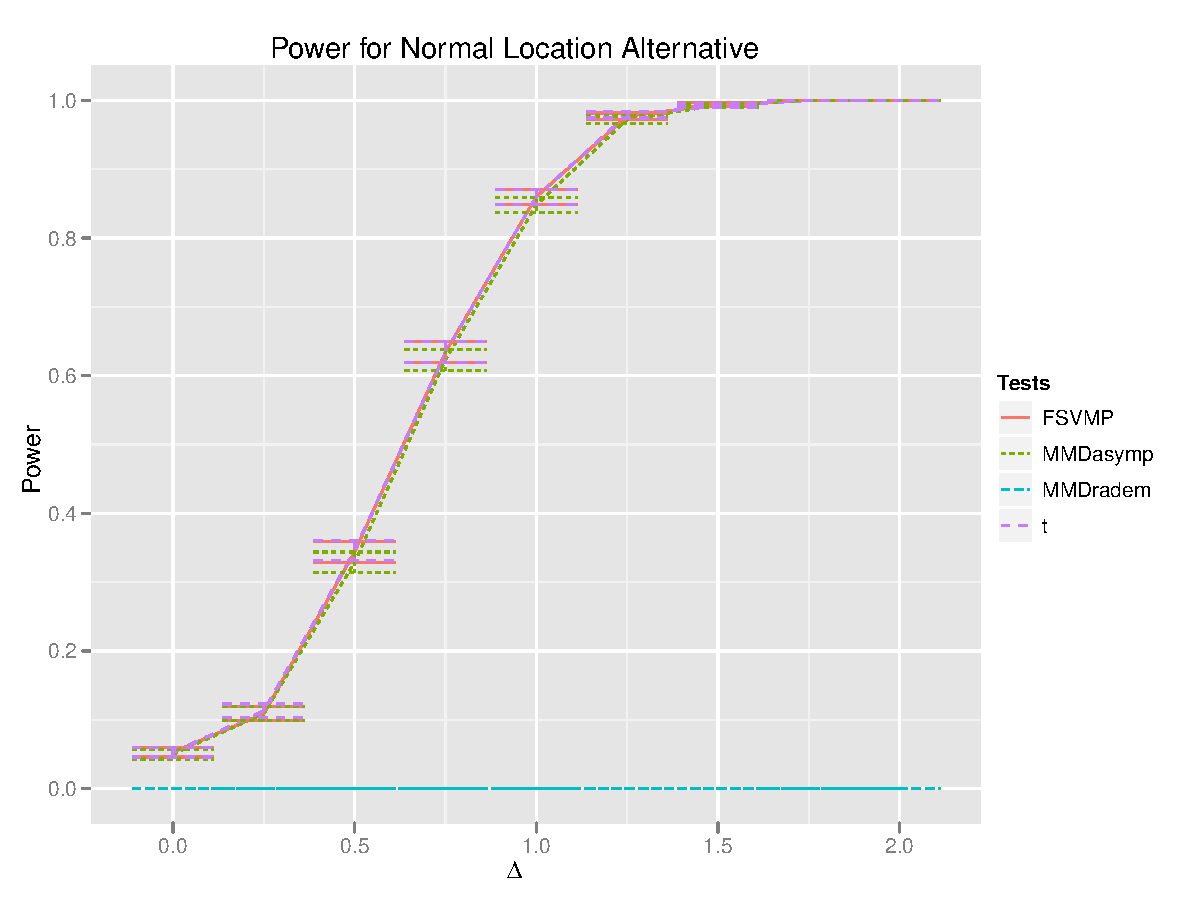
\includegraphics[width=.8\linewidth]{nips1.pdf}
  \caption{We see that the MMD statistic based on the asymptotic
    approximation (MMDasymp) has power similar to the $t$-test (t) and
    Friedman Test (FSVMP).  The MMD test based on the large deviations
  bound (MMDradem) is too conservative for small samples, failing to
  reject at all.  The other tests are seen to have level .05.  The
  error bars indicate two standard errors.}
\end{figure}

For a string data comparison, we consider Twitter data and look at the
latest 1,000 tweets from Barack Obama (@BarackObama) and Sarah Palin
(@SarahPalinUSA) obtained from the {\bf R} package {\bf twitteR} \cite{twitteR}.  We pre-process each tweet by removing all
hyperlinks and anything that is neither a letter nor a space.
Finally, we convert all letters to lowercase.  For simplicity, we
choose the $k$-spectrum kernel with $k=4$ \cite{leslie2002spectrum}
as our kernel for both KMMD and FSVMP.  Thus, each string is mapped to
a $27^4$ dimensional feature vector of counts of the number of 4
letter and space combinations.  We draw samples of various sizes from
both the Barack Obama tweets and Sarah Palin tweets in order to
empirically determine the power.  Again, the large deviations based
MMD test is too conservative, but this time the asymptotic
approximation is too aggressive and always rejects.  The FSVMP has
power approximately equal to its level for small samples, with power
eventually approaching 1.  

\begin{figure}[h!]
  \centering
  \includegraphics[width=.8\linewidth]{nips2.pdf}
  \caption{We see that the MMDasymp always rejects.  At these smaller sample
    sizes, the test is too sensitive and does not have level
    $\alpha=.05$.
    MMDradem is again too conservative for small samples, failing to
  reject at all.  The FSVMP has power equal to
  $\alpha=.05$ for small samples, with power approaching 1 for larger samples.
The error bars indicate two standard errors.}
\end{figure}

Lastly, we test draws from the same distribution, Barack Obama's
tweets, in order to determine empirically what the significance levels
of the tests are.  Only the SVMP is seen to have level consistent with
its design value of $\alpha=.05$.

\begin{figure}[h!]
  \centering
  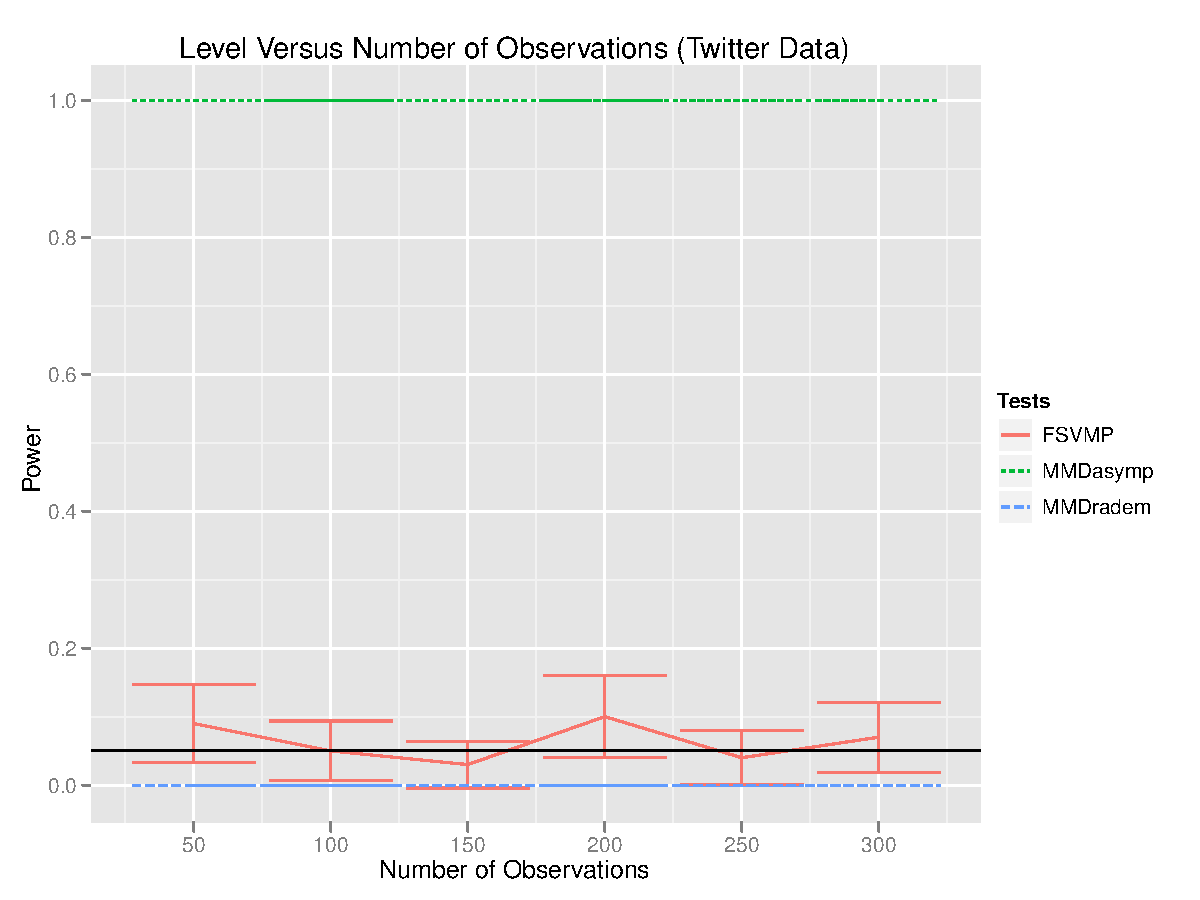
\includegraphics[width=.8\linewidth]{nips3.pdf}
  \caption{We draw i.i.d. samples with replacement from the same
    distribution (the 1,000 Barack Obama tweets).  The number of
    observations given is per sample, so we first compare 50 Barack
    Obama tweets with 50 Barack Obama tweets.  The error bars indicate
  two standard errors, and the horizontal line has y-intercept .05.
  We see that the MMDasymp always rejects, the MMDradem never rejects,
and the FSVMP has the correct level.}
\end{figure}

\section{Extensions}
Since the FSVMP is a kernel based test, it possesses all of the
advantages of other kernel procedures, in particular, data
integration.  Given heterogeneous data, as long as we can identify a
kernel with each type of data, there exist ways to optimally combine
this information.  For example, given kernel matrices $K_1,\ldots,
K_n$, the problem of optimizing the SVM criterion over weights
$\alpha_1,\ldots,\alpha_n$ to yield a new, optimal kernel
$K=\alpha_1K_1,\ldots,\alpha_nK_n$ can be framed as a semidefinite
program \cite{lanckriet2004learning}.  

In this way, the FSVMP can be extended to deal with heterogeneous
data.  So instead of just
fitting an SVM with one kernel matrix, the extra step is to optimize
the SVM criterion over the $n$ matrices.  The theoretical null distribution is unknown, so the
computational overhead lies in solving a new semidefinite program for
each permutation in order to make inference.  

\section{Summary}
We have coupled the Friedman Test with an SVM and have shown that with
a linear kernel, the FSVMP is a generalization of the permutation
$t$-test.  We have compared the FSVMP to two earlier tests based on the
MMD, a large deviations test and an asymptotic approximation test.
The FSVMP performs comparably to the $t$-test and the MMD test in a
simple univariate setting, where the MMD empirically has the right
operating characteristics, in particular, is of level $\alpha$.  

Because of its permutation design, the FSVMP always has level
$\alpha$, no matter the sample size.  We have highlighted this feature
with the Twitter data example in comparison with the MMD, which in
this small sample setting is overly aggressive in rejecting the null
hypothesis.  In future work, we hope to determine the theoretical null
distribution or at least be able to approximate it so that we can
bypass the permutation step.  Further, we would like to compare the
FSVMP to the improved MMD test of \cite{gretton2010fast}.

Finally, we have suggested an extension of the FSVMP to two-sample
testing with data integration.  Given possibly disparate data types and
kernels and an optimal way to combine data, the test extends in a
simple fashion.  The extra overhead is in the combination process for
each permutation.  The permutations are necessary for inference because the null
distribution in this case is unknown and probably quite complicated.  

\bibliographystyle{ieeetr}
\bibliography{ncray}
\end{document}
